\id{IRSTI 52.13.17}

{\bfseries MODERNIZATION OF GOLD-BEARING ORE EXTRACTION TECHNOLOGY
DEPENDING ON GEOLOGICAL AND MINING CONDITIONS}

\begin{figure}[H]
	\centering
	
\includegraphics[width=0.8\textwidth]{media/gorn2/image1}
	\caption*{}
\end{figure}

\textsuperscript{2}A.M.
\begin{figure}[H]
	\centering
	
\includegraphics[width=0.8\textwidth]{media/gorn2/image1}
	\caption*{}
\end{figure}


\emph{\textsuperscript{1} K.Kulazhanov named Kazakh University of
Technology and Business, Astana, Kazakhstan,}

\emph{\textsuperscript{2}Abylkas Saginov Karaganda Technical University,
Karaganda, Kazakhstan}

{\bfseries \textsuperscript{\envelope }}Correspondent-author:
\emph{assalamm@mail.ru.}

The article presents options for modernizing the technology for
extracting gold-bearing ore, depending on geological and mining
conditions, and discusses various technological solutions to improve
technologies. Based on review, analysis and generalization in specific
geological and mining conditions, the optimal width of the working site
was proposed. Continuous geotechnical monitoring should be carried out
at all stages of quarry development, including visual inspection of
slope conditions, crack mapping, and collection of deformation and
groundwater data. The following information should be recorded during
monitoring: geological characteristics of the slope,
engineering-geological characteristics for classifying the rock mass,
slope geometry, monitoring of damage as a result of drilling and
blasting operations, water seepage, quality and efficiency of cleaning,
monitoring of existing cracks and collapses.

Key words: mining technology, working platform width, bench height,
geotechnical monitoring, bench cleaning, gold-bearing ore.

{\bfseries ГЕОЛОГИЯЛЫҚ ЖӘНЕ ТАУ КЕН ТЕХНИКАЛЫҚ ЖАҒДАЙЛАРЫНА БАЙЛАНЫСТЫ
ҚҰРАМЫНДА АЛТЫН БАР КЕНДІ АЛУ ТЕХНОЛОГИЯСЫН ЖАҢҒЫРТУ}

{\bfseries \textsuperscript{1}Даулетжанова Ж.Т.,
\textsuperscript{2}А.М.Захаров\textsuperscript{\envelope },
\textsuperscript{2}Шмидт-Федотова И.М.}

\emph{\textsuperscript{1} Қ.Құлажанов атындағы Қазақ технология және
бизнес университеті, Астана, Қазақстан,}

\emph{\textsuperscript{2}Әбілқас Сағынов атындағы Қарағанды техникалық
университеті, Қарағанды, Қазақстан,}

\emph{e-mail: assalamm@mail.ru.}

Мақалада геологиялық және тау-кен жағдайларына байланысты алтын кендерін
алу технологиясын модернизациялау нұсқалары келтірілген, технологияларды
жақсарту үшін әртүрлі технологиялық шешімдер қарастырылған. Нақты
геологиялық және тау-кен жағдайларында шолу, талдау және жалпылау
негізінде жұмыс алаңының оңтайлы ені ұсынылады. Карьерді дамытудың
барлық кезеңдерінде беткейлердің жай-күйін визуалды тексеруді,
жарықтарды картаға түсіруді, деформациялар мен жер асты сулары бойынша
деректерді жинауды қамтитын үздіксіз геотехникалық мониторинг жүргізілуі
тиіс. Мониторинг кезінде мынадай ақпарат тіркелуі тиіс: борттың
геологиялық сипаттамалары, тау жыныстары массивін жіктеуге арналған
инженерлік-геологиялық сипаттамалар, борттың геометриясы, бұрғылау-жару
жұмыстарының нәтижесінде жойылуларды бақылау, судың ағуы, тазалаудың
сапасы мен тиімділігі, бар жарықтар мен құлауларды бақылау.

Түйінді сөздер: өндіру технологиясы, жұмыс алаңының ені, жиектің
биіктігі, геотехникалық мониторинг, жиектерді тазарту, құрамында алтын
бар кен.

{\bfseries МОДЕРНИЗАЦИЯ ТЕХНОЛОГИИ ВЫЕМКИ ЗОЛОТОСОДЕРЖАЩЕЙ РУДЫ В
ЗАВИСИМОСТИ ОТ ГЕОЛОГИЧЕСКИХ И ГОРНОТЕХНИЧЕСКИХ УСЛОВИЙ}

{\bfseries Ж.Т. Даулетжанова,
\textsuperscript{2}А.М.Захаров\textsuperscript{\envelope }, \textsuperscript{2}
И.М.Шмидт-Федотова}

\emph{\textsuperscript{1}Казахский университет технологии и бизнеса
им.К.Кулажанова, г. Астана, Казахстан,}

\emph{\textsuperscript{2}Карагандинский технический университет имени
Абылкаса Сагинова, г. Караганда, Казахстан,}

\emph{e-mail: assalamm@mail.ru.}

В статье приведены варианты модернизации технологии выемки
золотосодержащей руды в зависимости от геологических и горнотехнических
условий, рассмотрены различные технологические решения для улучшения
технологий. На основе обзора, анализа и обобщения в конкретных
геологических и горнотехнических условиях предложена оптимальная ширина
рабочей площадке. На всех этапах разработки карьера должен проводиться
непрерывный геотехнический мониторинг, включающий в себя визуальный
осмотр состояния откосов, картирование трещин, сбор данных по
деформациям и подземным водам. При мониторинге должна фиксироваться
следующая информация: геологические характеристики борта,
инженерно-геологические характеристики для классификации массива пород,
геометрия борта, наблюдение за разрушениями в результате буровзрывных
работ, просачивание воды, качество и эффективность зачистки, наблюдения
за имеющимися трещинами и обрушениями.

{\bfseries Ключевые слова:} технология добычи, ширина рабочей площадки,
высота уступа, геотехнический мониторинг, зачистка уступов,
золотосодержащая руда.

{\bfseries Introduction.} Novodneprovskaya territory is located 40-70 km
southwest of the city of Shchuchinsk. The area of the geological
allotment is 44.3 square km.

Within the geological allotment, two isolated gold-bearing ore fields
are distinguished - Novodneprovskoe and Raigorodskoe, which includes the
Northern Raygorodok and Southern Raygorodok gold-bearing deposits.

Industrial development of the Northern Raygorodok deposit has been
ongoing since 2010, and the Southern Raygorodok deposit since 2015.
Oxidized ores of the deposits are processed by heap leaching.

Open-pit mining of oxidized and mixed ores is carried out. The climate
of the area is sharply continental with dry and cool summers (with some
hot days) and cold, with prolonged frosts and strong winds in winter.

The described area belongs to the North Kazakhstan gold-bearing
province, which is a product of tectonic and magmatic events that
occurred during accretionary collision processes in the early Caledonian
period on the eastern border of the ancient Kokchetav massif and the
Seletino-Stepnyak system of island arcs of the early Paleozoic. An
important role in these processes was played by the processes of
redistribution and concentration of metals from Precambrian rocks and
island arcs. The Northern and Southern Raygorodok gold-bearing deposits
are a type of porphyry-epithermal ore-magmatic system in the
accretionary continental margin. The Raigorod ore field is confined to
the volcanotectonic structure of the same name.

In regional terms, the work area is located in the border area between
two large first-order structures - the Kokchetav middle massif and the
Teniz depression, which are fundamentally different in geological
structure and development history.

This led to the complex geological structure of the area, intense
magmatism and widespread development of faults. Weathering crusts of
areal and linear types are widely developed in the area of the deposit.
The thickness of the areal weathering crusts reaches 70 m, linear (in
the eastern part of the deposit) 120-180 m. The boundary of the oxidized
ore zone follows the boundary of the weathering crust and is located at
depths of about 40-100 m, which made it possible to mine the first stage
of the quarry with a depth of up to 80-100 m without the use of drilling
and blasting operations. In stockwork bodies, the two noted
morphological types often accompany each other in various combinations
and combinations {[}1, 2{]}. Ore zones and bodies have a linear
morphology with a steep dip.

The length of individual ore bodies varies from tens to 645 m, and
thickness - from a meter to 65 m, while vein-like ore bodies usually
have an insignificant thickness of up to 3 m and a small extent (up to
100 m) with pinching out along strike and dip.

The depth of mineralization exceeds 750-850 m, and with depth there is
no tendency for ore bodies to pinch out, and the gold content increases.

{\bfseries Materials and Methods.} There is a certain pattern in the
distribution of ore bodies - the center of the mineralized strip is
maximally saturated with closely spaced ore bodies of irregular shape,
on the flanks they are less common and spatially separated. This is
explained by the development of a predominantly stockwork type in the
center, and vein and isolated stockwork type on the flanks. The gold
content changes literally at a distance of the first meters {[}3{]}.

Extraction unit is the smallest economically and technologically optimal
section of a deposit with a reliable calculation of initial reserves
(block, panel, longwall, part of a ledge), the development of which is
carried out by a unified development system and technological scheme of
extraction, according to which the most accurate separate accounting of
production can be carried out in terms of quantity and quality of
minerals {[}4,5{]}.

Taking into account the peculiarities of the geological structure of the
deposit, the most optimal excavation unit will be a ledge (horizon) with
a height of 7.5 m, during the development of which it will be possible
to most accurately ensure the accounting, condition and movement of
reserves, losses and dilution.

The concept of a ledge - as an excavation unit corresponds to the
definition and functions of a minimum section and meets the requirements
for an excavation unit, because:

- economically and technologically justified optimal mining geometric
unit by the project;

- with reliable calculation of initial ore reserves;

- development of which is carried out by a unified development system
and technological scheme of excavation;

- by which an accurate separate accounting of the extraction of ore mass
can be carried out according to the quantity and content of metal
(useful component) in it {[}6{]}.

For each mining unit, the subsoil user creates a passport reflecting the
state and movement of mineral reserves, the actual fulfillment of loss
and dilution indicators, and the state of mining operations.

The provision of a quarry with ore reserves and volumes of overburden
ready for extraction are expressed for the period of operation in months
or fractions of a year, based on its planned productivity in the next
year; When putting capacity into operation, the availability of the
quarry is calculated: for minerals - based on the amount of capacity
introduced and introduced in the next year, for overburden rocks - based
on the planned productivity for overburden rocks for the coming year.

With year-round operation, the quarry' s supply is:

- ready-to-excavate ore reserves -- at least 2.5 months;

- volumes of overburden rock ready for excavation - at least 2.5 months;

- volumes of loose overburden ready for excavation - at least 1.8
months.

Based on the design capabilities of the adopted type of equipment, the
height of the working benches is assumed to be 7.5 m.

The calculated value of the minimum permissible width of working
platforms under standard conditions was determined taking into account
the regulations for the placement of the excavator entry, the width of
the shoulders, safety strips and the safety shaft was 50 m (Figure 1)
{[}7{]}.

\begin{figure}[H]
	\centering
	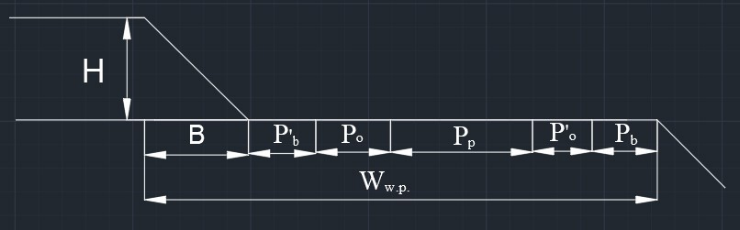
\includegraphics[width=0.8\textwidth]{media/gorn2/image18}
	\caption*{}
\end{figure}


{\bfseries Fig. 1 - Working platform width}

The width of the working platform is determined by the formula:

Ww.p.= B+Pp+Pо+P' о+Pb+ P' b, m

where B - Full width of rock collapse after explosion;

P'{}\textsubscript{b} - Width of the safety strip between
the first row of wells and the edge;

P\textsubscript{о} - Upland shoulder width;

P\textsubscript{p} - Roadway width;

P\textsubscript{' о} - Downstream curb width;

P\textsubscript{b} - Collapse prism width.

When driving entry and cutting trenches, as well as when working in
difficult, cramped conditions, working with a dead-end face is used
{[}8{]}.

The width of a dead-end face, as a rule, corresponds to two excavator
radii. If the width of the dead-end face is less than two digging radii,
the possibility of turning the excavator and safely placing vehicles in
the trench is checked. The turning radius and length of the dump truck
must correspond to unimpeded entry and loading at the face.

{\bfseries Results and Discussion.} In areas prone to deformation, it is
recommended to carry out blasting operations in a gentle or controlled
mode. Blasting can have a significant and often decisive impact on the
behavior of slopes. Drilling and blasting with a controlled perimeter is
recommended for all sides of the final pit contour provided for in the
project. Controlled perimeter drilling and blasting technologies must be
developed and their effectiveness verified before the beads are formed
to the final design position {[}9{]}. The performance of each controlled
explosion must be monitored and analyzed to ensure it remains consistent
with changing conditions.

An important factor in ensuring the stability of the pit walls is the
management of groundwater pressure. Groundwater pressure inside the edge
and along structural differences can increase destabilizing
(destructive) forces. These forces can be mitigated by using appropriate
measures. Measures to reduce pressure in slopes should include the
installation of drainage ditches. To stabilize slopes, wells for pumping
water around the perimeter and horizontal drainages are recommended
{[}10{]}.

An important activity is clearing the ledges. Cleaning involves removing
suspended rocks from the surface of the slopes and subsequent cleaning
at the base of the slope. Cleaning should be the final operation of each
excavation cycle when constructing both permanent and temporary pit
walls. This procedure allows you to maintain order and reduce the risk
of rock collapse.

At all stages of quarry development, continuous geotechnical monitoring
should be carried out, including visual inspection of the condition of
slopes, mapping of cracks, collection of data on deformations and
groundwater.

Information collected during monitoring should be documented and
processed by a competent geotechnical professional. When monitoring, the
following information should be recorded: geological characteristics of
the wall (lithology, deformation, weathering), engineering-geological
characteristics for classifying the rock mass, geometry of the wall
(including deformations and factors causing them), observation of damage
as a result of drilling and blasting operations, water infiltration,
quality and efficiency of cleaning, monitoring of existing cracks and
collapses.

The opening of the designed quarries is carried out using both external
and internal entrance trenches.

The design of the opening scheme in quarries is carried out taking into
account a number of conditions and factors, including: ensuring the
minimum range of hauling the rock mass along intra-quarry roads with
ensuring a minimum volume of overburden in the contours of the quarries;
locations of ore stockpiles and overburden dumps.

The opening of each new horizon is carried out depending on the
parameters of the section of the ore zone to be mined by creating a
temporary dead-end or permanent ramp in a place convenient for the
unhindered development of its reserves and preparing the site for
opening a new underlying horizon.

{\bfseries Conclusion.} At all stages of quarry development, continuous
geotechnical monitoring should be carried out, including visual
inspection of the condition of slopes, mapping of cracks, collection of
data on deformations and groundwater. In areas prone to deformation, it
is recommended to carry out blasting operations in a gentle or
controlled mode. An important activity is clearing the ledges. Cleaning
involves removing suspended rocks from the surface of the slopes and
subsequent cleaning at the base of the slope. Cleaning should be the
final operation of each excavation cycle when constructing both
permanent and temporary pit walls. This procedure allows you to maintain
order and reduce the risk of rock collapse.

\emph{{\bfseries Financing.} This research was funded by the Committee of
Science of the Ministry of Science and Higher Education of the Republic
of Kazakhstan (Grant No.BR24993009).}

{\bfseries References}

1. Volkov M.A. Izuchenie fiziko-mekhanicheskikh svoistv gornykh porod na
raznykh etapakh razrusheniya. / M.A. Volkov, D.V. Solov'ev, L.A. Belina,
A.G. Pimonov. // Vestnik Kuzbasskogo gosudarstvennogo tekhnicheskogo
universiteta. 2017. S. 16-19. {[}in Russian{]}

2.Kazakov N.N., Viktorov S.D., Shljapin A.V.,Lapikov I.N. Droblenie
gornyh porod vzryvom v kar' erah.Droblenie gornyh porod
vzryvom v kar' erah : monografija / Kazakov N.N. {[}i
dr.{]}. --- M.: RAN, 2020 -520 s. (s.404-404) ISBN 978-5-907036-96-3.
{[}in Russian{]}

3.Rakishev B.R. Vzaimosvyaz' mezhdu sistemoi i tekhnologiei otkrytoi
razrabotki poleznykh iskopaemykh. // Gornyi zhurnal Kazakhstana. 2017.
№1. S.20-27. {[}in Russian{]}

4.Delentas A., Benardos А., Nomikos P. Analyzing Stability Conditions
and Ore Dilution in Open Stope Mining// Mineral resources.- 2021.-
Vol.1(12). - P.1404. \href{https://doi.org/10.3390/min11121404}{DOI
10.3390/min11121404}

5.Potapov M.G. Ekologicheskaya otsenka tekhnologicheskikh skhem
otkrytykh gornykh rabot. // Gornyi zhurnal. -2003. - № 3.- S. 81-86.
{[}in Russian{]}

6.Akishev A.N. Upravlenie razvitiem rabochei zony kimberlitovykh
kar'erov. / A.N. Akishev, V.A. Bakhtin, E.V. Bondarenko, S.L. Babaskin.
// Gornaya promyshlennost'.- 2004.- №1.- S. 53-59. {[}in Russian{]}

7. Vuyeykova O., Sładkowski A., Stolpovskikh I., Akhmetova M.:
Rationalization of

road transport park for the carriage of mining rocks in the open mines.
// Transport Problems Volume 11 Isuee 1. P 79-85, Poland, Gliwice 2016,
ISSN 1896-0596 IF 0,265
http://transportproblems.polsl.pl/en/default.aspx

8.Shakenov A., A. Sładkowski, I. Stolpovskikh. Haul road condition
impact on tire life of mining dump
truck//\href{https://www.researchgate.net/journal/Naukovyi-Visnyk-Natsionalnoho-Hirnychoho-Universytetu-2223-2362?_tp=eyJjb250ZXh0Ijp7ImZpcnN0UGFnZSI6InB1YmxpY2F0aW9uIiwicGFnZSI6InB1YmxpY2F0aW9uIn19}{Naukovyi
Visnyk Natsionalnoho Hirnychoho Universytetu}.-2022. - Vol.192(6)- P.
25-29. DOI
\href{http://dx.doi.org/10.33271/nvngu/20226/025}{10.33271/nvngu/20226/025}

9.Kadnikova O.,Kuzmin S., Altynbayeva G., Turbit A., Khabdullina Z.
Development of a New Environmentally-Friendly Technology for
Transportation of Mined Rock in the Opencast Mining. // Environmental
and Climate Technologies.- 2020.-Vol. 24(1).- P.341-356 DOI
10.2478/rtuect-2020-0019

10.Kalyuzhny A.S. Opredelenie parametrov narushennoj zony i ob''emov
potencial'nyh vyvalov dlya uslovij kar'era «Olenij ruchej»//Gornyj
informacionnoanaliticheskij byulleten.- 2016.- No.7.- S. 403-412. {[}in
Russian{]}

\emph{{\bfseries Information about the authors}}

Dauletzhanova Zh.T.-PhD, Associate Professor of the Department of
Chemistry, Chemical Technology and Ecology, K.Kulazhanov named Kazakh
University of Technology and Business, Astana, Kazakhstan, e-mail:
kaliyeva\_zhanna@mail.ru;

Zakharov A.M. - master of Technical Sciences, senior lecturer at the
Department of Mineral Deposit Development, Abylkas Saginov Karaganda
Technical University, Karaganda, Kazakhstan, e-mail: assalamm@mail.ru;

Shmidt-Fedotova I.M. -- PhD, lecturer of the Department of «Development
Mineral Deposit», Abylkas Saginov Karaganda Technical University,
Karaganda, Kazakhstan, irinka.shmidt@mail.ru

\emph{{\bfseries Сведения об авторе}}

Даулетжанова Ж.Т. - PhD, ассоциированный профессор кафедры «Химия,
химическая технология и экология», Казахский университет технологии и
бизнеса имюК.Кулажанова, г. Астана, Казахстан, e-mail:
kaliyeva\_zhanna@mail.ru;

Захаров А.М. - магистр технических наук, старший преподаватель кафедры
«Разработка месторождений полезных ископаемых», Карагандинский
технический университет имени Абылкаса Сагинова, г. Караганда,
Казахстан, e-mail:
\href{mailto:assalamm@mail.ru}{\nolinkurl{assalamm@mail.ru}};

Шмидт-Федотова И.М.- PhD, преподаватель кафедры «Разработка
месторождений полезных ископаемых», Карагандинский технический
университет имени Абылкаса Сагинова, (г. Караганда, Казахстан),
irinka.shmidt @mail.ru.